\section{Introduction}
 The correlation algorithms considered thus far are useful only when there are exactly two
datasets.  However, in many applications, we may have access to multiple datasets of high
dimensional features that we believe contain correlated signals. Access to more
than two datasets arises in applications such as handwritten digit classification
\cite{yu2007learning}, multi-temporal hyperspectral imaging \cite{nielsen2002multiset},
and medical imaging \cite{correa2010canonical, deleus2011functional}.

The theory of multiset canonical correlation analysis (MCCA) has evolved over the past
decades. The earliest work on extending CCA to three datasets was conducted by Vinograde
\cite{vinograde1950canonical}. This work found the canonical form of the three dataset
correlation matrix but made no attempts at finding the canonical vectors. In
\cite{steel1951minimum}, Steel considers the particular objective function of minimizing
the generalized variance between the canonical variates of an arbitrary number of
datasets. In 1961, Horst first considered the practical problem of fusing features from
multiple datasets \cite{horst1961relations,horst1961generalized}. He provides a solution
for two particular objective functions originally called the ``maximum correlation
method'', which is now called the sum of correlations method, and the ``rank one
approximation method'', which is now called the maximum variance method. A decade later,
Kettenring \cite{kettenring1971canonical} considered a more general extension of
Hotellings's \cite{hotelling1936relations} original CCA work. He considers five objective
functions that extend CCA to multiple datasets. Each objective function represents
some notion of multiset correlation. All five formulations of multiset CCA return canonical
vectors for each dataset and correlation coefficients and each reduce to CCA when only
two datasets are present. Two decades later, Nielsen \cite{nielsen1994analysis} extended
Kettenring's analysis by also considering four constraint functions placed on the
canonical vectors in the optimization problem.

The five objective functions posed by Kettenring and four constraint functions posed by
Nielsen give rise to twenty different optimization problems and thus twenty different
formulations of MCCA. In this section, we consider all twenty such optimization
problems. We begin by deriving the theoretical solution to each of these, unifying the
works above and completing any formulations previously unsolved. As the performance of
empirical MCCA has not previously been studied, we also derive empirical versions of each
MCCA formulation using training data SVDs of each dataset. In Appendix
\ref{sec:mcca_derivs}, we derive a solution to each of the twenty optimization problems
formed by choosing one objective function and one constraint function. We then consider
empirical version of each MCCA formulation.

We then consider the performance of one particular optimization problem, MAXVAR. We show
that, similar to empirical CCA, the solution to this problem is a SVD of matrix with block
entries of the pairwise product of right singular vectors of the individual datasets. We
then apply the same principles used in ICCA to develop an informative version of MAXVAR,
which we call IMCCA. Using the idea of trim-then-fuse, we propose to trim all data SVDs to
include only the \textit{informative} singular vectors. We provide some analysis of the
behavior of these algorithms and provide a test statistic to use to determine the number
of correlations present in multiple datasets. We discuss why multi-dataset correlation
analysis is difficult but showcase on a real world dataset that IMCCA greatly outperforms
MAXVAR and can robustly identify sources of correlation.


\section{Mathematical Formulation of MCCA}



Let $y_1,y_2,\dots,y_m$ be observations drawn from $m$ distributions $y_i\sim
\mathcal{Y}_i$ with $y_i\in\complex^{d_i}$. Assume, without loss of generality, that $y_i$
is zero mean. Define the covariance between distributions as $\E{y_iy_j^T}=R_{ij}$ for
$i,j=1,\dots,m$. Define the joint observation vector $y$ and its covariance $R=\E{yy^H}$ as
\be
y = \left[\begin{array}{c}y_1\\ \vdots \\ y_m\end{array}\right] \in\complex^{d\times 1},\,\,\,\,R
= \left[\begin{array}{ccc}R_{11}&\dots&R_{1m}\\ \vdots&\ddots&\vdots\\ 
    R_{m1}&\dots&R_{mm}\end{array}\right]\in\complex^{d\times d}
\ee
where $d=\sum_{i=1}^md_i$.

The goal of MCCA is to find canonical coefficient vectors, $x_i\in\complex^{d_i\times 1}$
for $i=1,\dots,m$, such that the canonical variates, $w_i=x_i^Hy_i$, are optimal with
respect to an objective function $J(\cdot)$ and constraint function $h(\cdot)$. We
consider five objective functions \cite{kettenring1971canonical} in Section
\ref{sec:obj_func} and four constraints functions \cite{nielsen1994analysis} in Section
\ref{sec:constraints}. Define the vector of canonical vectors as
$x=\left[x_1^H,\dots,x_m^H\right]^H\in\complex^{d\times 1}$ and the vector of canonical
variates as $w=[w_1,\dots,w_m]^H\in\complex^{m\times 1}$. The covariance matrix of $w$ is
\begin{equation*}
\Phi(x)=\E{ww^H}=\left[\begin{array}{ccc} x_1^HR_{11}x_1 & \dots & x_1^HR_{1m}x_m \\ \vdots
    & \ddots & \vdots \\ x_m^HR_{m1}x_1 & \dots & x_m^HR_{mm}x_m\\ \end{array}\right].
\end{equation*}
Using this notation, the MCCA optimization problem is
\begin{equation}\label{eq:chpt10:opt_prob}
\begin{aligned}
&\underset{x}{\mathop{\rm optimize}} && J(\Phi(x))\\
&\text{subject to} && h(x,R).\\
\end{aligned}
\end{equation}

\subsection{Constraint Functions, $h(x,R)$}\label{sec:constraints}
In \cite{nielsen2002multiset,nielsen1994analysis}, Nielsen describes four constraints
placed on the canonical vectors that are natural to use in MCCA. Using our notation and
new naming scheme, these constraint functions are:

\begin{description}
\item[a)] \textbf{NORM} - The canonical coefficient vectors each have unit norm.
  \begin{equation*}
    h(x,R) = x_i^Hx_i=1,\, 1\leq i\leq m
  \end{equation*}
  This objective function has the same flavor as other machine learning algorithms such as
  PCA.

\item[b)] \textbf{AVGNORM} - The vector of canonical vectors, $x$, has unit norm.
  \begin{equation*}
    h(x,R) = x^Hx=\sum_{i=1}^mx_i^Hx_i = 1
  \end{equation*}

\item[c)] \textbf{VAR} - The canonical variates each have unit variance.
  \begin{equation*}
    x_i^HR_{ii}x_i = 1,\, 1\leq i\leq m.
  \end{equation*}
  This is the natural extension of the CCA constraint functions. 

\item[d)] \textbf{AVGVAR} - The canonical variates have average variance of $1/m$. 
  \begin{equation*}
    \sum_{i=1}^mx_i^HR_{ii}x_i =1.
  \end{equation*}
  This may be written $\Tr(X^H RX ) = 1$, where $X = \blkdiag(x_1,\dots,x_m)$. 
\end{description}


\subsection{Objective Functions, $J(\Phi(x))$}\label{sec:obj_func}

In \cite{kettenring1971canonical}, Kettenring describes five objective functions, each
used to detect a different form of linear relationship among the datasets. Under the VAR
and AVGVAR constraints above, each of the objective functions reduces to the standard CCA
formulation and thus the standard CCA solution. Using our notation, these objective
functions are:

\begin{enumerate}
\item \textbf{SUMCORR} - Maximize the sum of the correlations between each of the canonical variates.
  \begin{equation*}
    J(\Phi(x)) = \max_{x_1,\dots,x_m} \sum_{i=1}^m\sum_{i=1}^m x_i^HR_{ij}x_j=\max_{x_1,\dots,x_m}\ones^H\Phi(x) \ones 
  \end{equation*}
  This is the natural extension of the CCA objective function. It  was first proposed by
  Horst in \cite{horst1961relations}. 

\item \textbf{SSQCORR} - Maximize the sum of the squares of the correlations between
  each of the canonical variates.
  \begin{equation*}
    J(\Phi(x)) = \max_{x_1,\dots,x_m}\sum_{i=1}^m\sum_{j=1}^m(x_i^HR_{ij}x_j)^2=
    \max_{x_1,\dots,x_m}\|\Phi(x)\|_F^2 =
    \max_{x_1,\dots,x_m}\sum_{i=1}^m\lambda_i^2(\Phi(x)). 
  \end{equation*}

  where $\lambda_i$ are the eigenvalues of $\phi(x)$. This is very similar to SUMCORR
  except that it penalizes small pairwise correlations more than SUMCORR does. Under the
  VAR constraint, the $m\times m$ identity matrix is the least informative $\Phi(x)$ as
  this denotes no correlation between any of the canonical variates. Therefore, we want
  $\Phi(x)$ to be as different as possible from the identity matrix. Under the VAR
  constraint, this is what the SSQCORR objective function accomplishes. It was first
  proposed in 1971 by Kettenring \cite{kettenring1971canonical}.

\item \textbf{MAXVAR} - Maximize the largest eigenvalue of $\Phi$, $\lambda_1(\Phi(x))$.
  \begin{equation*}
    J(\Phi(x)) = \max_{x_1,\dots,x_m}\lambda_1(\Phi(x))
  \end{equation*}
  MAXVAR was created by Horst in \cite{horst1961relations} to find the canonical vectors
  that give $\Phi(x)$ the best approximation (in the Frobeneus norm) to a rank-1
  matrix. Horst's original name for this method was the ``rank one approximation
  method''. The corresponding largest eigenvalue, $\lambda_1(\Phi(x))$ is a notion of
  variance and thus the new name.

\item \textbf{MINVAR} - Minimize the smallest eigenvalue of $\Phi$, $\lambda_m(\Phi(x))$.
  \begin{equation*}
    J(\Phi(x)) = \min_{x_1,\dots,x_m}\lambda_d(\Phi(x))
  \end{equation*}
  Instead of maximizing the energy in the top eigenvalue, we wish to minimize the energy
  in the last eigenvalue. In \cite{bach2003kernel}, MINVAR is shown to have the desired
  property that the minimal eigenvalue has a fixed range in $[0,1]$ whereas the maximal
  eigenvalue found by MAXVAR has a range dependent on the dimensions of the variables. It
  was first proposed in 1971 by Kettenring \cite{kettenring1971canonical}.

\item \textbf{GENVAR} - Minimize the generalized variance of $w$, which is equivalent to
  minimizing the determinant of the correlation matrix of $w$.
  \begin{equation*}
    J(\Phi(x)) = \min_{x_1,\dots,x_m}\left|\Phi(x)\right| = \min_{x_1,\dots,x_m}\prod_{i=1}^m\lambda_i(\Phi(x))
  \end{equation*}
  This is the oldest of the five criterion and was proposed by Steel in 1951
  \cite{steel1951minimum}. This seems to involve a tradeoff between choosing $x$ to have
  large leading eigenvalues and small tail eigenvalues.
\end{enumerate}

\begin{table*}[h!]
  \centering
  \begin{tabular}{ll}
    \midrule
    $y_i$ & Observation from dataset $i$ \\
    $y$ &  $[y_1^H,\dots,y_m^H]^H$\\ 
    $d_i$ & $\text{Dimension of } y_i$ \\
    $d=\sum_{i=1}^md_i$& $\text{Dimension of } y$\\ 
    $m$ & $\text{Number of datasets}$ \\
    $n$ & $\text{Number of observations}$\\ 
    $x_i\in\complex^{d_i}$ & $\text{Canonical coefficient vector}$ \\
    $x\in\complex^d$ & $[x_1^H,\dots,x_m^H]^H$\\ 
    $w_i\in\complex$ & $\text{Canonical variate}$\\
    $w\in\complex^m$ & $[w_1,\dots,w_m]^H$\\ 
    $X\in\complex^{d\times m}$ & $\blkdiag(x_1,\dots,x_m)$ \\
    $\Phi(x)$ &  $\text{Correlation matrix of }w$\\ 
    $R_D\in\complex^{d\times d}$ & $\blkdiag(R_{11},\dots,R_{mm})$\\
    $R\in\complex^{d\times d}$ & $\text{Matrix of } [R_{ij}]_{ij}$\\ 
    $\widetilde{R}(x)\in\complex^{d\times d}$ & $\text{Matrix of}
    [(x_i^HR_{ij}x_j)R_{ij}]_{ij}$ \\
    $Y_i\in\complex^{d_i\times n}$ & Training data matrix\\
    $U_i\in\complex^{d_i\times d_i}$ & $\text{Left singular vectors of } Y_i$\\
    $U\in\complex^{d\times m}$ & $\blkdiag(U_1,\dots,U_m)$\\ 
    $\Sigma_i\in\complex^{d_i\times n}$ & $\text{Singular values matrix of }$ $Y_i$\\
    $\Sigma\in\complex^{d\times nm}$ & $\blkdiag(\Sigma_1,\dots,\Sigma_m)$\\ 
    $V_i\in\complex^{n\times n}$ & $\text{Right singular vectors of } Y_i$\\
    $V\in\complex^{n\times nm}$ & $[V_1,\dots,V_m]$\\ 
    $\Lambda\in\complex^{m\times m}$ & Diag matrix of Lagrange multipliers\\
    $\Lambda_D\in\complex^{d\times d}$ & $\blkdiag\left(\lambda_1 I_{d_1},\dots,\lambda_m
      I_{d_m}\right)$\\  
    $\widetilde{\Sigma}\in\complex^{d\times d}$ & $\blkdiag(\Sigma_1(:,1:d_1),\dots
    \Sigma_m(:,1:d_m))$\\ 
    $\widetilde{V}\in\complex^{n\times  d}$&$[V_1(:,1:d_1),\dots,V_m(:,1:d_m)]$ \\
    $\ones$ & $\left[1,\dots,1\right]$\\
    \midrule
  \end{tabular}
  \caption{Notation used in MCCA}
  \label{tab:mcca_notation}
\end{table*}

\section{Theoretical and Empirical MCCA Derivations}

In this section, we provide a solution for each of the twenty MCCA formulations based on
the five objection functions described in Section \ref{sec:obj_func} and four constraint
functions described in Section \ref{sec:constraints}. Some of these solutions have been
previously reported in \cite{kettenring1971canonical, nielsen1994analysis}. We complete
the analysis and unify the results. We provide the empirical solution for each algorithm
provided training data matrices $Y_1,\dots, Y_m$. In such a setting, we are given $n$
samples (observations) from each data distribution. Using these $n$ samples, we form $m$
 training data matrices by stacking the observations as columns in a
matrix. We denote these training data matrices $Y_1=\left[y_1^{(1)},\dots
  y_1^{(n)}\right]\in\complex^{d_1\times n},\dots, Y_m=\left[y_m^{(1)},\dots,
  y_m^{(n)}\right]\in\complex^{d_m\times n}$. 

For all empirical derivations, we assume that we are given $n$ samples in each training
dataset. We denote the SVD of each training dataset as $Y_i=U_i\Sigma_iV_i^H$ and form the
matrices $U\in\complex^{d\times d}=\blkdiag(U_1,\dots,U_m)$, $\Sigma\in\complex^{d\times
  nm}=\blkdiag(\Sigma_1,\dots,\Sigma_m)$, and $V\in\complex^{n\times nm}=[V_1,\dots,V_m]$.
Using these data SVDs, we form sample covariance matrices,
$\widehat{R}_{ij}=\frac{1}{n}Y_iY_j^H = \frac{1}{n}U_i\Sigma_iV_i^HV_j\Sigma_j^HU_j^H$
with which we form $\widehat{R}=U\Sigma V^HV\Sigma^HU^H$ and
$\widehat{R}_D=U\Sigma\Sigma^HU^H$. Please refer to Table \ref{tab:mcca_notation} for a
summary of the notation used throughout the MCCA derivations.

The derivations are provided in Appendix \ref{sec:mcca_derivs}. Table
\ref{tab:main_results} in the following section summarizes the solution to each
problem. It assigns a number-letter pair to each MCCA optimization problem (1-5 for the
objective function, a-d for the constraint function). This label can be used to look up
the appropriate derivation in Appendix \ref{sec:mcca_derivs}. The table provides the
appropriate eigen-system used to solve the problem if all the covariance matrices are
known. The table also provides the appropriate eigen-system used to solve the problem in
the empirical setting where we are given training datasets to estimate unknown covariance
matrices. The last column in the table provides references that use, discuss, or derive
the MCCA formulation.

\subsection{Manopt Software for Optimization on Manifolds}

Many of the problems discussed in Appendix \ref{sec:mcca_derivs} do not yield closed form
solutions because either the cost function is unwieldy or because the constraint functions
complicate the derivations. For these problems we use the Manopt software provided at
\textit{www.manopt.org}. The Manopt software specializes in solving constrained optimization
problems when the constraints are manifolds. This software package is able to solve
nonlinear optimization problems. For reference, see \cite{boumal2013manopt}. To use the
solvers, we must provide a cost function and its associated gradient.

All of our constraints will be of the form $\|x\|=1$ where $x\in\reals^{p}$. The
associated manifold that we use for this constraint is the sphere manifold called via
\texttt{spherefactory(p,1)}. If we have multiple of such constraints, then we use the
\texttt{productmanifold} to ensure all constraints are satisfied. See the Manopt
documentation and provided code for an example. 

After selecting the appropriate manifold and providing the cost and gradient functions, we
use the \texttt{trustregions} solver to find a solution for our problems. This returns the
minimized cost and the point that achieved the minimum cost. If our objective
function has a cost function that seeks a maximum, we provide the negative of the
true cost function and the gradient is computed from this negative cost. 

\subsection{Successive Canonical Vectors}

The derivations in Appendix \ref{sec:mcca_derivs} show how to compute the first stage
canonical vectors and canonical correlation. We may compute $r=\min(d_1,\dots,d_m,n)$
canonical vector and correlation pairs. We use the standard constraint on successive
canonical variates
\be
\E{w_i^{(k)}w_i^{(k-j)}} = 0,\,\, \text{ for } j=1,\dots,k-1,\,\,\,\forall i.
\ee
Here, the subscript $i$ indexes the canonical variates and the superscript $(k)$ indexes
the stage of the canonical vector and correlation pair. This requires the next stage
canonical variates to be uncorrelated to all previous canonical variates for a given
dataset. Using the definition for canonical variates, this constraint becomes
\be
\E{x_i^{(k)H}y_iy_i^Hx_i^{(k-j)}} = x_i^{(k)H}R_{ii}x_i^{(k-j)} = 0,\,\, \text{ for }
j=1,\dots,k-1,\,\,\,\forall i. 
\ee
To enforce this constraint, we run the following algorithm
\begin{enumerate}
\item Form $X\in\complex^{d\times mk}=\blkdiag(X_1,\dots,X_m)$ where $X_i = [x_i^{(1)},\dots,x_i^{(k)}]$
\item Project the canonical vectors onto $R_D$ via $B = R_DX \in\complex^{d\times mk}$
\item Compute a basis for the span of $B$ via the rank-$k$ SVD, $B=U_B\Sigma_B V_B^H$
\item Form the projection matrix onto the orthogonal completment of this basis $P = I -
  U_BU_B^H$
\item Project the training data onto $P$ via $\widetilde{Y} = PY$
\item Recompute covariance matrices used in optimization using $\widetilde{Y}$
\end{enumerate}

\subsection{MCCA Summary}\label{sec:summary}

Table \ref{tab:main_results} summarizes the solution to each of the twenty optimization
problems and shows for which ones we must use the Manopt software package and which ones
we have closed form solutions in terms of eigen-systems.  All of the empirical eigenvalue
systems rely on the matrix product $V^HV$. This is wonderful news because it directly
makes contact with the similar $V_x^HV_y$ matrix used in CCA. In Chapter 4 we saw that by
trimming this matrix to only include informative singular vectors of the individual
datasets we can greatly improve correlation detection. This observation will drive our
derivation of IMCCA. We note that in this thesis we only do so for MAXVAR, but this $V^HV$
matrix appears in many of the optimization problems and other such informative versions of
these algorithms are within reach. Many of the SUMCORR and SSQCORR theoretical
eigen-systems are non-normal, using multiple Lagrange multipliers. Some of these problems
can be solved with Manopt, however, some result in non-unique solutions. Obviously, such
formulations of MCCA should be avoided.

\begin{table*}[!h]
\small
  \centering
  \begin{tabular}{lllllll}\toprule
    \# & $J(x)$ & $h(x,R)$  & Eigenvalue Prob & Empirical Prob & Ref\\
    \midrule
    1a & SUMCORR & NORM & $R \widetilde{x} = \Lambda_D\widetilde{x}$ & Manopt &
    \cite{nielsen2002multiset,nielsen1994analysis}\\ 
    &&&$x = \Lambda_{\widetilde{x}}\widetilde{x}$ &&\\
    1b & SUMCORR & AVGNORM & $R x = \rho x$ &
    $\widehat{R}\widehat{x} = \widehat{\rho}\widehat{x}$&
    \cite{nielsen1994analysis}\\ 
    1c & SUMCORR & VAR & $R\widetilde{x}=\Lambda_DR_D\widetilde{x}$  & Manopt&
    \cite{nielsen2002multiset,kettenring1971canonical,nielsen1994analysis}\\
    &&&$x = R_D^{-1/2}\Lambda_{\widetilde{x}}\widetilde{x}$&&\\
    1d & SUMCORR & AVGVAR &  $R_D^{-1/2}RR_D^{-1/2}\widetilde{x}=\rho\widetilde{x}$&
    $\widetilde{V}^T\widetilde{V}\widehat{f}=\widehat{\rho}\widehat{f}$ &
    \cite{deleus2011functional,nielsen2002multiset,via2005canonical}\\ 
    &&&$x=R_D^{-1/2}\widetilde{x}$&$\widehat{x}=U\widetilde{\Sigma}^{-1}\widehat{f}$&
    \cite{nielsen1994analysis,yu2007learning}\\  
    \midrule
    2a & SSQCORR & NORM & $\widetilde{R}(x)x = \Lambda_Dx$ & Manopt &
    \cite{nielsen1994analysis}\\  
    2b & SSQCORR & AVGNORM & $\widetilde{R}(x)x = \lambda x$ & Manopt &
    \cite{nielsen1994analysis}\\ 
    2c & SSQCORR & VAR & $\widetilde{R}(x)x= \Lambda_DR_Dx$ & Manopt &
    \cite{correa2010canonical,kettenring1971canonical,nielsen1994analysis}\\ 
    2d & SSQCORR & AVGVAR & $\widetilde{R}(x)x=\lambda R_Dx$ & Manopt&
    \cite{nielsen1994analysis}\\ 
    \midrule
    3a & MAXVAR & NORM & $R\tilde{a} = \rho\tilde{a}$ &
    $\widehat{R} \widehat{f}=\widehat{\rho} \widehat{f}$&
    \cite{nielsen1994analysis}\\ 
    &&&$x=\Lambda_{\tilde{a}}^{-1}\tilde{a}$&
    $\widehat{x}=\Lambda_{\widehat{f}}^{-1}\widehat{f}$ &\\ 
    3b & MAXVAR & AVGNORM & $x_i=u_{1i}$ &
    $\widehat{x}_i = u_{1i}$ &
    \cite{nielsen1994analysis}\\ 
    3c & MAXVAR & VAR &
    $R_D^{-1/2}RR_D^{-1/2}\tilde{a}=\rho\tilde{a}$&
    $\tilde{V}^H\tilde{V}\widehat{f}=\widehat{\rho}\widehat{f}$&
    \cite{kettenring1971canonical,nielsen1994analysis}\\ 
    &&&$x=R_D^{-1/2}\Lambda_{\widetilde{a}}^{-1}\widetilde{a}$&
    $\widehat{x}=U\widetilde{\Sigma}^{-1}\Lambda_{\widehat{f}}^{-1}\widehat{f}$&\\ 
    3d & MAXVAR & AVGVAR &
    Non-unique &
    Non-unique &
    \cite{deleus2011functional,via2005canonical,nielsen1994analysis}\\ 
    &&& $x=u_i/\sigma_i$ & $\widehat{x} = u_i/\sigma_i$&\\  
    \midrule
    4a & MINVAR & NORM & $R\tilde{a} = \rho_{\text{min}}\tilde{a}$ &
    $\widehat{R}\widehat{a}=\widehat{\rho}_{\text{min}}\widehat{a}$&  
    \cite{nielsen1994analysis}\\ 
    &&&$x=\Lambda_{\widetilde{a}}^{-1}\widetilde{a}$&
    $\widehat{x}=\Lambda_{\widehat{a}}^{-1}\widehat{a}$ &\\  
    4b & MINVAR & AVGNORM & Non-unique & Non-unique & 
    \cite{nielsen1994analysis}\\ 
    &&& $x_i = u_{1i}$ & $\widehat{x}_i = u_{1i}$&\\
    4c & MINVAR & VAR &
    $R_D^{-1/2}RR_D^{-1/2}\widetilde{a}=\rho_{\text{min}}\widetilde{a}$&
    $\widetilde{V}^H\widetilde{V}\widehat{f}=\widehat{\rho}_{\text{min}} \widehat{f}$&
    \cite{kettenring1971canonical,nielsen1994analysis}\\ 
    &&&$x=R_D^{-1/2}\Lambda_{\widetilde{a}}^{-1}\widetilde{a}$&
    $\widehat{f}=U\widetilde{\Sigma}^{-1}\Lambda_{\widehat{f}}\widehat{f}$& \\
    4d & MINVAR & AVGVAR & Non-unique & Non-unique&
    \cite{nielsen1994analysis,bach2003kernel}\\ 
    &&& $x=u_{i}/\sigma_i$ & $\widehat{x} = u_i/\sigma_i $&\\  
    \midrule
    5a & GENVAR & NORM & Non-eigen prob & Manopt&  \cite{nielsen1994analysis}\\
    5b & GENVAR & AVGNORM & Non-eigen prob & Manopt&  \cite{nielsen1994analysis}\\
    5c & GENVAR & VAR &Non-eigen prob & Manopt&
    \cite{kettenring1971canonical,nielsen1994analysis}\\  
    5d & GENVAR & AVGVAR & Non-eigen prob & Manopt &  \cite{nielsen1994analysis}\\
    \bottomrule
  \end{tabular}
  \caption{Summary of MCCA optimization problems. The objective functions are described in
    Section \ref{sec:obj_func}. The constraints are described in section
    \ref{sec:constraints}. The eigenvalue problem column is the theoretical solution while
    the Empirical problem column describes how to solve the problem given empirical
    data. All eigenvalue problems solve for the maximum eigenvalue-eigenvector pair
    except for the MINVAR problems, which solves for the minimum eigenvalue-eigenvector
    pair. The final column lists references which describe the MCCA optimization
    problem. }\vskip-0.2cm 
  \label{tab:main_results}
\end{table*}


\section{Proposed Informative MCCA Algorithm}

We choose to focus our attention on two of the above problems, 3c and 4c, MAXVAR and
MINVAR with the VAR constraint. We choose to examine these because they are a very natural
extension from CCA. One can show that each of the objective functions is equivalent to the
CCA objective function when $m=2$. To draw a natural connection from CCA to MAXVAR, we
first recall that the canonical correlations of empirical CCA are exactly the singular
values of 
\beq\label{eq:chpt10:C_cca}
C=V_1^HV_2,
\eeq
where $V_1$ and $V_2$ are the right singular vectors of the data matices $Y_1$ and $Y_2$,
respectively. Define the SVD of $C=FKG^H$. Consider the matrix 
\beq\label{eq:chpt10:R_cca}
R_{\text{cca}} = \left[\begin{array}{c}V_1^H\\V_2^H\end{array}\right]\left[\begin{array}{cc}V_1 &
    V_2\end{array}\right] = \left[\begin{array}{cc}I_{d_1} &
    V_1^HV_2\\ V_2^HV_1 & I_{d_2}\end{array}\right].
\eeq
As shown in \cite{bach2003kernel}, $R$ has eigenvalues that come in pairs
\be
\left\{1+k_i,1-k_i,\right\}.
\ee
More specifically, the eigenvalue decomposition of $R_{\text{cca}}$ is
\be
R_{\text{cca}} = \left[\begin{array}{cc}F & -F\\ G & G\end{array}\right]
\left[\begin{array}{cc}I + \left(KK^H\right)^{-1/2} & 0\\ 0 & I - \left(K^HK\right)^{-1/2}\end{array}\right]
\left[\begin{array}{cc}F & -F\\ G & G\end{array}\right]^H.
\ee
From the eigenvalue decomposition of this matrix, we can exactly recover the canonical
correlations $k_i$ and the needed transformations $F$ and $G$. These transformations appear
in a very specific block structure. Each eigenvector contains the corresponding block
components of the transformation for each dataset. In addition, just as the eigenvalues come in pairs, the
eigenvectors come in pairs. Comparing the eigenvectors corresponding to the eigenvalues
$1+k_i$ and $1-k_i$ we see that the component corresponding to the second dataset is the
same while the component of the first dataset simply changes sign. 

Therefore, the CCA solution by taking the SVD of $C$ in \ref{eq:chpt10:C_cca} is equivalent to
maximizing the largest $\min(d_1,d_2)$ eigenvalues of $R$ in (\ref{eq:chpt10:R_cca}). However, we
can also uncover the same solution by minimizing the smallest $\min(d_1,d_2)$ eigenvalues
of $R$ as well. We note that the CCA optimization problem explicitly uses the VAR
constraint function. 

From this discussion it is clear that MAXVAR and MINVAR using the VAR constraint are
extremely natural extensions for the CCA optimization problem. We simply concatenate the
right singular vectors of any additional datasets to the matrix product in
(\ref{eq:chpt10:R_cca}) to form 
\beq\label{eq:chpt10:R_mcca}
\Rmcca =
\left[\begin{array}{c}V_1^H\\V_2^H\\\vdots\\V_m^H\end{array}\right]\left[\begin{array}{cccc}V_1
    & V_2 & \cdots & V_m\end{array}\right] = \left[\begin{array}{cccc}I_{d_1} & 
    V_1^HV_2 & \cdots & V_1^HV_m\\ V_2^HV_1 & I_{d_2}& \cdots & V_2^HV_m\\
  \vdots & \vdots & \ddots & \vdots \\ V_m^HV_1 & V_m^HV_2 & \cdots & I_{d_m}\end{array}\right].
\eeq
If our datasets are completely noise free, then examining the eigenvalues of $\Rmcca$
directly gives us the correlation structure. Any eigenvalues $k_i\neq 1$ represent correlated
components. We can have at most 
\be
r = \left\lfloor{\frac{\sum_{i=1}^md_i}{2}}\right\rfloor
\ee
correlations. Having this many number of correlated components would require all
correlations to be pair-wise. 

Interpreting the eigenvalues and eigenvectors of $\Rmcca$ is much more complicated than
CCA. While any eigenvalue not equal to 1 conveys a correlation between datasets, the
strength of this correlation is coupled with the eigenvector structure. Consider the
following examples both for $m=3$ and $d_1=d_2=d_3=1$
\be
\Rmcca^{(1)} =  \left[\begin{array}{ccc}1 &  1 & 0\\ 1 & 1&0\\  0 & 0 &
    1 \end{array}\right],\,\,\,\, \Rmcca^{(2)} =  \left[\begin{array}{ccc}1 &  0.5 & 0.5\\ 0.5 &
    1&0.5\\  0.5 & 0.5 & 1 \end{array}\right].
\ee
$\Rmcca^{(1)}$ corresponds to a setting where the only component of dataset 1 and 2 are
perfectly correlated and dataset 3 is independent. $\Rmcca^{(2)}$ corresponds to the
setting where all three components are weakly mutually correlated. However, the largest
eigenvalue of both of these matrices is 2. This eigenvalue is not one so it represents
correlation in our datasets. However, the structure of our correlation is very different.

To determine the structure of our correlation, we must examine the associated eigenvectors
of $\Rmcca$. The eigenvectors corresponding to the largest eigenvalues of these matrices
are
\be
u^{(1)} = \frac{1}{\sqrt{2}}\left[1, 1, 0\right]^T,\,\,\,\,u^{(2)} = \frac{1}{\sqrt{3}}\left[1,1,1\right]^T.
\ee
From these eigenvectors, we directly can see the correlation structure revealed by the
eigenvector. This ambiguity in correlation structure is never a problem in vanilla CCA as
there are only two datasets. Components are either correlated or they are not and so the
eigenvalue in CCA directly gives our correlation structure and we can determine our
necessary transformations directly from the eigenvectors. In MAXVAR, after determining
that our eigenvalue represents a correlation, we then need to inspect the corresponding
eigenvector to determine the correlation structure.

Similar to the result by \cite{pezeshki2004empirical}, we would like to determine when the eigenvalues
returned by empirical MAXVAR erroneously represent false correlation. In CCA, we had the
result that when $n<d_1+d_2$, $k_1=1$ deterministically. For MAXVAR and MINVAR, we provide
the following two Theorems and Conjecture.

\begin{Th}\label{th:maxvar}
If $2n<\min_{i\neq j\neq k}(d_i+d_j+d_k)$ then the largest eigenvalue of $\Rmcca$ is equal
to $m$. 
\end{Th}
\begin{proof}
  By definition, $V_i$ is a $n\times d_i$ matrix. Without loss of generality, let $V_i$ be
  ordered such that $d_1\leq d_2\leq d_m$. When $n<d_1+d_2$, then $V_1$ and $V_2$ must
  span a shared subspace of dimension $d_1+d_2-n$. By a similar geometric argument, this
  shared subspace of dimension $d_1+d_2-n$ will intersect the span of $V_3$ if 
  \be
  (d_1+d_2-n) + d_3 > n.
  \ee
  Re-arranging terms means that 
  \be
  d_1+d_2+d_3 > 2n
  \ee
  implies that $V_1$, $V_2$ and $V_3$ all span a common subspace of dimension
  $(d_1+d_2+d_3) - 2n$. In this setting we have that $d_1+d_2>n$ and $d_1+d_2+d_3>2n$
  which implies that $d_3>n$. Therefore for any $i>3$, $d_i>n$. By induction, we have that 
  for any $i>3$, $V_i$ will intersect the common subspace of dimension $(d_1+d_2+d_3)-2n$
  if
  \be
  (d_1+d_2+d_3 -2n) + d_i > n,
  \ee
  which holds if $d_i>n$, which we just showed was true. Therefore, when 
  \be
  2n <\min_{i\neq j\neq k}(d_i+d_j+d_k)
  \ee
  all $V_i$ span a common subspace of at least dimension 1. 

  With this observation in mind, we may write
  \be
  V_i = \left[q \,\,\,\,\,q_i^\perp\right]
  \ee
  where $q$ is a basis vector for this shared subspace and $q_i^\perp$ is the orthogonal
  complement representing the rest of $V_i$. With this definition, we have that for any
  $i\neq j$, 
  \be
  V_i^HV_j = \left[\begin{array}{cc}1 & 0 \\ 0 & Q_{ij}\end{array}\right],
  \ee
  where $Q_{ij} = \left(q_i^\perp\right)^Hq_j^\perp$. With this block structure we can
  observe that the first column and row of $\Rmcca$ is 
  \be
  w = \left[e_1^H,e_2^H,\dots,e_m^H\right]^H,
  \ee
  where $e_i^H = [1,0,\dots,0]\in\complex^{1\times d_i}$. Therefore, it is clear that
  $\frac{1}{m}w$ is an eigenvector of $\Rmcca$ associated with the eigenvalue $m$.  
\end{proof}

\begin{Th}\label{th:minvar}
If $n<\sum_{i=1}^md_i$ then the smallest eigenvalue of $\Rmcca$ is zero.
\end{Th}
\begin{proof}
  We provide a short proof by simply geometric and rank arguments. Recall that $V_i\in\complex^{n\times
    d_i}$. Then
  \be
  V = \left[\begin{array}{c}V_1^H\\V_2^H\\\vdots\\V_m^H\end{array}\right]
  \ee
  is a $\sum_{i=1}^md_i \times n$ matrix. When $n<\sum_{i=1}^md_i$, this matrix can have a
  maximum rank of $n$. Therefore
  \be
  \rank(\Rmcca) = \rank(V^HV) \leq n < \sum_{i=1}^md_i.
  \ee
  Therefore, $\Rmcca$ is not full rank and has at least 1 zero-eigenvalue. As $\Rmcca$ is
  symmetric positive semi-definite, the smallest eigenvalue is therefore zero.
\end{proof}

\begin{Conj}\label{conj:minmaxvar}
We conjecture that when $n<\sum_{i=1}^md_i$, the largest eigenvalue of $\Rmcca$ is
determined entirely based on $n$ and $\sum_{i=1}^md_i$ and not on the underlying
correlation.
\end{Conj}

The intuition behind Conjecture \ref{conj:minmaxvar} is based on the observation from CCA
that the eigenvalues of $R_{\text{cca}}$ come in pairs
$\left\{1+k_i,1-k_i\right\}$. MAXVAR returns the eigenvalues above 1 and MINVAR returns
the eigenvalues below 1. However, unlike in CCA, the eigenvalues of $C_{\text{mcca}}$ are
not symmetric about 1 and so we do not have an elegant closed form relationship. Our
intuition leads us to believe that these eigenvalues of $\Rmcca$ are coupled and represent
the same correlation structure. Theorem \ref{th:maxvar} states that if we are in a certain
sample deficient regime, the largest eigenvalues are deterministic. Similarly, Theorem
\ref{th:minvar} states that in a different sample deficient regime, the smallest
eigenvalues are deterministic. These sample deficient regimes are different for the
largest and smallest eigenvalues; the regime is larger for the smaller
eigenvalues. Therefore, due to the hypothesized coupling of the largest and smallest
eigenvalues we believe Conjecture \ref{conj:minmaxvar} holds. In this setting, like in
empirical CCA, we conjecture that the canonical vectors are simply random and we would not
like to use them in an algorithm.

\subsection{Low-Rank Multi-dataset Model}

Let $y_1^{(i)}\in\complex^{d_1\times 1},\dots,y_m^{(i)}\in\complex^{d_m\times 1}$ be
modeled as 
\beq\label{eq:chpt10:mcca_data_model} 
y_j^{(i)} = U_js_j^{(i)} + z_j^{(i)}
\eeq
where for $j=1,\dots,m$, $U_j^HU_j=I_{k_j}$ $z_j^{(i)}\simiid\mathcal{CN}(0,I_{d_j})$. Furthermore, assume that 
\be
s_j^{(i)}\simiid\mathcal{CN}(0,\Theta_j)\\
\ee
where
$\Theta_j=\diag\left(\left(\theta_j^{(1)}\right)^2,\dots,\left(\theta_j^{(k_j)}\right)^2\right)$. Assume
that for all $i$ and $j$, $z_j^{(i)}$ are mutually independent and independent 
from all $s_j^{(i)}$. Finally, assume that 
\be
\E{s_j^{(i)} s_\ell^{(i)H}} \defeq K_{j\ell} = \Theta_j^{1/2}P_{j\ell}\Theta_\ell^{1/2}
\ee
where the entries of $P_{j\ell}$ are between $-1$ and $1$ and represent the correlation
between the entries of $s_j$ and $s_\ell$. For reasons to be made clear later, for
$j,\ell=1,\dots,m$ define 
\be
\widetilde{K}_{j\ell} = \left(\Theta_j+I_{d_j}\right)^{-1/2}K_{j\ell}\left(\Theta_\ell+I_{d_\ell}\right)^{-1/2}.
\ee
 Under this model, we define the following 
covariance matrices  
\beq\label{eq:chpt10:mcca_true_scm}\ba
&\E{y_jy_j^H} = U_j\Theta_jU_j^H+I_{d_j} \defeq R_{jj}\\
&\E{y_jy_\ell^H} = U_jK_{j\ell}U_\ell^H \defeq R_{j\ell}.\\
\ea\eeq

With this model we have that our target matrix in MAXVAR is
\be
\Rmcca =R_D^{-1/2}RR_D^{-1/2}\\
\ee
where
\be\ba
&R &&= \E{\left[\begin{array}{c} y_1^{(i)}\\y_2^{(i)}\\ \vdots \\
      y_m^{(i)}\end{array}\right] \left[\begin{array}{cccc} y_1^{(i)H} & y_2^{(i)H} & \cdots &
        y_m^{(i)H}\end{array}\right]}\\
&&& = \left[\begin{array}{cccc} R_{11} & 
    R_{12} & \cdots & R_{1m}\\ R_{21} & R_{22}& \cdots & R_{2m}\\
  \vdots & \vdots & \ddots & \vdots \\ R_{m1} & R_{m2} & \cdots & R_{mm}\end{array}\right]\\
\ea\ee
and
\be
R_D = \blkdiag(R_{11},R_{22},\dots,R_{mm}).
\ee
With these definitions, the block diagonal elements of $\Rmcca$ are $I_{d_j}$ and the
block off-diagonal elements are $R_{jj}^{-1/2}R_{j\ell}R_{\ell\ell}^{-1/2}$. Using our
model in (\ref{eq:chpt10:mcca_data_model}), we have that
\be\ba
& R_{jj}^{-1/2}R_{j\ell}R_{\ell\ell}^{-1/2} && =
\left(U_j\Theta_jU_j^H+I_{d_j}\right)^{-1/2}U_jK_{j\ell}U_\ell^H\left(U_\ell\Theta_\ell U_\ell^H+I_{d_\ell}\right)^{-1/2}\\
&&& =  U_j\left(\Theta_j +
  I_{d_j}\right)^{-1/2}K_{jk}\left(\Theta_\ell+I_{d_\ell}\right)^{-1/2}U_\ell^H\\
&&& = U_j\widetilde{K}_{j\ell}U_\ell^H.
\ea\ee
Therefore, by defining $U = \blkdiag(U_1,\dots,U_m)$, we have that
\be
\Rmcca = U\underbrace{\left[\begin{array}{cccc} I_{k_1} & 
    \widetilde{K}_{12} & \cdots & \widetilde{K}_{1m}\\ \widetilde{K}_{21} & I_{k_2}& \cdots & \widetilde{K}_{2m}\\
  \vdots & \vdots & \ddots & \vdots \\ \widetilde{K}_{m1} & \widetilde{K}_{m2} & \cdots & I_{k_m}\end{array}\right]}_{\widetilde{K}}U^H.
\ee
Finally, let $U_{\widetilde{K}}K_{\widetilde{K}}U^H_{\widetilde{K}}$ be the eigenvalue
decomposition of $\widetilde{K}$ where
\be
K_{\widetilde{K}}=\diag(\kappa_1,\dots,\kappa_k),
\ee
 where $k=\sum_{j=1}^mk_j$. The number
of correlated components is thus equal to the number of eigenvalues of $\Rmcca$ that are
greater than one,
\be
\text{\# of correlated components} \defeq t = \sum_{i=1}^k\indicator_{\left\{\kappa_i > 1\right\}}.
\ee

\subsection{Informative MCCA}

In many applications, however, we do not know the covariance matrices
$R_{j\ell}$. Therefore, we cannot determine the number of correlated components by
examining the rank of $\Rmcca$. Instead, we are given multiple snapshots from
(\ref{eq:chpt10:mcca_data_model}) that we stack columnwise into data matrices
\be
Y_j = \left[y_j^{(1)},\dots,y_j^{(n)}\right].
\ee
Using these data matrices, we form estimates of the unknown covariance matrices via
\be
\widehat{R}_{j\ell} = \frac{1}{n}Y_jY_\ell^H.
\ee
Define the data SVDs as
\be
Y_j  = \widehat{U}_j\widehat{\Sigma}_j\widehat{V}_j^H,
\ee
the trimmed matrices as
\be\ba
& \widetilde{U}_j = \widehat{U}_j(:,1:\min(d_j,n))\\
& \widetilde{U}_j = \widehat{V}_j(:,1:\min(d_j,n)),
\ea\ee
and the matrices
\be
\widetilde{U} = \blkdiag(\widetilde{U}_1,\dots,\widetilde{U}_m),\,\,\,\,\widetilde{V} =
\left[\widetilde{V}_1,\dots \widetilde{V}_m\right] .
\ee
Empirical MAXVAR examines the eigen-decomposition of the matrix
\be
\Rmccahat = \widetilde{U}\widetilde{V}^H\widetilde{V}\widetilde{U}.
\ee
Define the eigenvalues of this matrix as
$\widehat{\kappa}_1,\dots,\widehat{\kappa}_d$,which are the
MAXVAR estimates of the correlations present in the multiple datasets. MAXVAR may return
up to a maximum of
\be
r = \left\lfloor{\frac{\sum_{i=1}^md_i}{2}}\right\rfloor
\ee
correlations. However, based on the model in (\ref{eq:chpt10:mcca_data_model}), we know that our
datasets are low-rank and it is common to return 
\be
\widehat{r} = \left\lfloor{\frac{\sum_{i=1}^m\widehat{k}_i}{2}}\right\rfloor
\ee
where $\widehat{k}_j$ are estimates of the number of underlying signals in each dataset.

In the spirit of the ICCA algorithm and motivated by the low-rank data model in
(\ref{eq:chpt10:mcca_data_model}), we propose the following informative version of MAXVAR. We
know that not all right singular vectors are informative and so we trim our data matrices
\be\ba
& \Ucir_j = \widehat{U}_j\left(:,1:\widehat{k}_j\right)\\
& \Vcir_j = \widehat{V}_j\left(:,1:\widehat{k}_j\right)
\ea\ee
and define
\be
\Ucir = \blkdiag(\Ucir_1,\dots,\Ucir_m),\,\,\,\,\Vcir =
\left[\Vcir_1,\dots \Vcir_m\right] .
\ee
Using these trimmed estimates, we define the informative MAXVAR (IMCCA) matrix as
\be
\Rmccatil = \Ucir\Vcir^H\Vcir\Ucir^H.
\ee
Define the eigenvalues of this IMCCA matrix as
$\widetilde{\kappa}_1,\dots,\widehat{\kappa}_{\widehat{r}}$. 

To estimate the number of correlated signals present in our datasets, we examining the
eigenvalues of the matrices $\Rmccahat$ and $\Rmccatil$. We know from the population model
that the number of eigenvalues above 1 represent correlations. Therefore, we can set a
threshold to estimate the number of correlations via
\beq\label{eq:chpt10:that}\ba
& \widehat{t}_{\text{mcca}}= \sum_{i=1}^{\widehat{r}} \indicator_{\left\{\widehat{\kappa}_1 > 1 + \tau_{\text{mcca}}^\alpha\right\}}\\
&\widehat{t}_{\text{imcca}} = \sum_{i=1}^{\widehat{r}}
\indicator_{\left\{\widehat{\kappa}_1 > 1 + \tau_{\text{imcca}}^\alpha\right\}}, 
\ea\eeq
where the thresholds $\tau_{\text{mcca}}^\alpha$ and $\tau_{\text{immca}}^\alpha$ are set to
achieve a desired false alarm rate $\alpha$.

Similar to the ICCA Theorems, we make the following two conjectures. 

\begin{Conj}
Let $d_1,\dots,d_m, n\to\infty$ with $d_j/n\to c_j$. Given the data model in
(\ref{eq:chpt10:mcca_data_model}), the IMCCA estimate of the number of correlated components in
(\ref{eq:chpt10:that}) converges to the actual number of correlated components under the following
condition
\be
\widehat{t}_{\text{imcca}}\convas t\,\,\,\,\text{ if }\, \forall j=1,\dots,m, \min_{i=1,\dots,k_j}\theta_j^{(i)} > c_j^{1/4}
\ee
\end{Conj}

\begin{Conj}
Consider the missing data setting where our the entries of our data matrices may only be
partially observed as
\be
Y_j = \left(U_j\Theta_j^{1/2}V_j^H+Z_j\right)\odot M_j
\ee
where
\be
M_{k\ell}^j = \begin{cases} 1 & \text{ with probability } \gamma_j\\ 0 & \text{ with
    probability } 1-\gamma_j \end{cases}.
\ee
Let $d_1,\dots,d_m,n\to\infty$ with $d_j/n\to c_j$. Then the estimated number of
correlated components in (\ref{eq:chpt10:that}) converges to the actual number of correlated
components under the following condition
\be
\widehat{t}_{\text{imcca}}\convas t\,\,\,\,\text{ if }\, \forall j=1,\dots,m, \min_{i=1,\dots,k_j}\theta_j^{(i)} > \frac{c_j^{1/4}}{\sqrt{\gamma_j}}
\ee
\end{Conj}


\section{Controlled Video-Video-Video Experiment}

To verify the effectiveness of IMCCA for real world applications, and to showcase the
extreme sub-optimality of empirical MCCA, we setup a controlled experiment consisting of
four stationary flashing lights and three stationary iPhone cameras. Figure
\ref{fig:chpt10:mcca_setup} shows the left, middle, and right camera views for one frame
of the video experiment. Figure \ref{fig:chpt10:mcca_sources} manually identifies each
source in each camera view by drawing a colored box around it. The left camera can see a
flashing laptop screen (L1), a flashing phone light (PH1), and a flashing tablet screen
(T1). The middle camera has only one source, the flashing tablet screen (T1). The right
camera can see the flashing tablet screen (T1), the flashing laptop screen (L1) via an
external monitor, and a flashing police light (PL1). We summarize these sources in Table
\ref{tab:mcca_descrp}. Based on our setup, all cameras share the T1 source, while the left
and right views share the L1 source. The left and right views also each have an
independent source in their view.

To synchronize the cameras we used the RecoLive MultiCam iPhone app
\footnote{http://recolive.com/en/}. After turning on all light sources, we recorded
20 seconds of video at 30 frames per second. The resolutions of the iPhone's cameras were
all $1920\times 1080$ pixels. 

\begin{figure}
  \begin{center}
    \subfigure[Left Camera]{
      \label{fig:chpt10:mcca_left}
      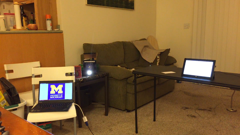
\includegraphics[width=0.3\textwidth]{chpt10_mcca/figs/mcca_left_color.png}
    }
    \subfigure[Middle Camera]{
      \label{fig:chpt10:mcca_mid}
      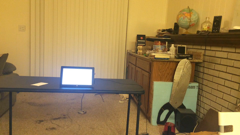
\includegraphics[width=0.3\textwidth]{chpt10_mcca/figs/mcca_mid_color.png}
    }
    \subfigure[Right Camera]{
      \label{fig:chpt10:mcca_right}
      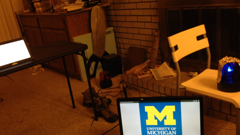
\includegraphics[width=0.3\textwidth]{chpt10_mcca/figs/mcca_right_color.png}
    }   
    \caption{Left, middle, and right camera views of our four sources for the controlled
      MCCA flashing light experiment.}
    \label{fig:chpt10:mcca_setup}
  \end{center}
\end{figure}

\begin{figure}
  \begin{center}
    \subfigure[Left Camera]{
      \label{fig:chpt10:mcca_man_left}
      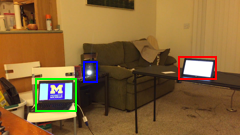
\includegraphics[width=0.3\textwidth]{chpt10_mcca/figs/mcca_left_man.png}
    }
    \subfigure[Middle Camera]{
      \label{fig:chpt10:mcca_man_mid}
      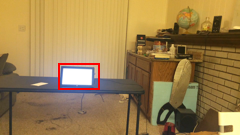
\includegraphics[width=0.3\textwidth]{chpt10_mcca/figs/mcca_mid_man.png}
    }
    \subfigure[Right Camera]{
      \label{fig:chpt10:mcca_man_right}
      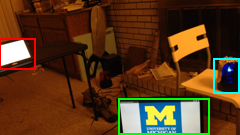
\includegraphics[width=0.3\textwidth]{chpt10_mcca/figs/mcca_right_man.png}
    }   
    \caption{Manual identification of each source in each camera. All three sources share
      a common flashing tablet, outlined in red. The left and right camera views share a
      common flashing laptop screen, outlined in green. The left camera has an independent
      flashing phone light, outlined in dark blue. The right camera has an independent
      flashing police light, outlined in cyan.}
    \label{fig:chpt10:mcca_sources}
  \end{center}
\end{figure}

\begin{table*}[h!]
\centering
\begin{tabular}{l|l}\toprule
Camera & Source\\
\midrule
Left & Laptop L1\\
& Phone PH1\\
& Tablet T1\\
\midrule
Middle & Tablet T1\\
\midrule
Right & Tablet T1\\
& Laptop L1 \\
& Police Light PL1\\
\bottomrule
\end{tabular}
\caption{Visual sources for each camera view. All three cameras share Tablet T1. The left
  and right cameras share Laptop L1. The left and right cameras each have an independent
  flashing light source.}
\label{tab:mcca_descrp}
\end{table*}

To post-process the video data, we first converted the video streams to grayscale and then
downsampled each spatial dimension by a factor of 8, resulting in a resolution of $240\times
135$. We then vectorized each image and stacked the 600 frames into data matrices, all
of dimension $32400 \times 600$. Finally, we subtract the mean from each dataset so that
we may run PCA, MCCA, and IMCCA on the zero-mean datasets, $Y_{\text{left}}$,
$Y_{\text{middle}}$, and $Y_{\text{right}}$.

First, we run PCA on the individual datasets $Y_{\text{left}}$, $Y_{\text{middle}}$, and
$Y_{\text{right}}$ to identify the signals residing in each dataset. We know from our
setup that the left and right cameras both have three sources. Figure
\ref{fig:chpt10:mcca_svs} plots the singular values of $Y_{\text{left}}$,
$Y_{\text{middle}}$, and $Y_{\text{right}}$. Figures \ref{fig:chpt10:mcca_pca_left},
\ref{fig:chpt10:mcca_pca_mid} and \ref{fig:chpt10:mcca_pca_right} plot the singular vector
heatmaps corresponding to the top 3 singular values of $Y_{\text{left}}$,
$Y_{\text{middle}}$, and $Y_{\text{right}}$, respectively. Each figure also overlays a
thresholded version of the singular vectors onto the raw video. The threshold that we use
is $\sqrt{\log(d_i)/d_i}$. From these figures, PCA does a good job at identifying the pixels
containing a signal (flashing light).

\begin{figure}
  \begin{center}
    \subfigure[Left Camera]{
      \label{fig:chpt10:mcca_left_sv}
      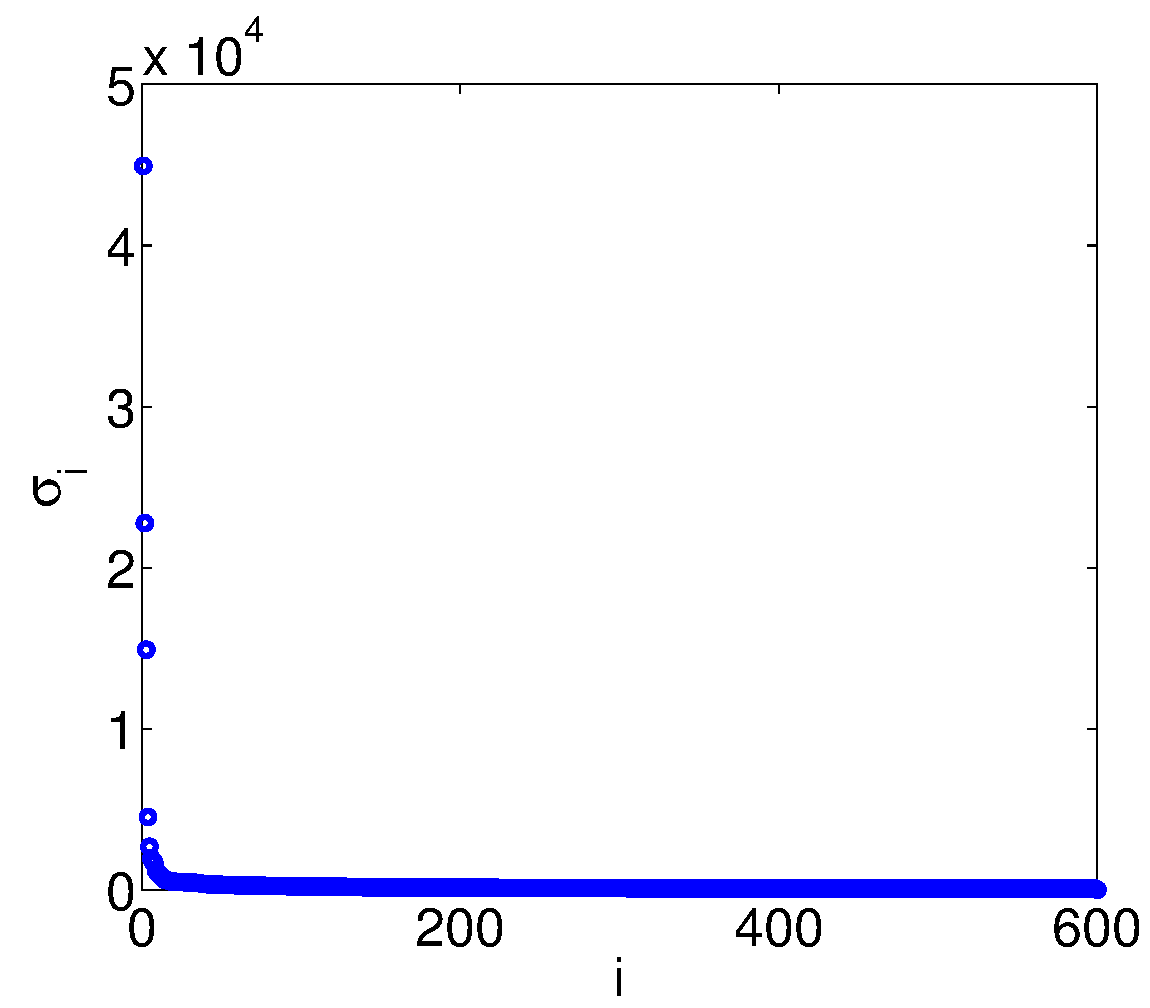
\includegraphics[width=0.3\textwidth]{chpt10_mcca/figs/mcca_lsv.pdf}
    }
    \subfigure[Middle Camera]{
      \label{fig:chpt10:mcca_mid_sv}
      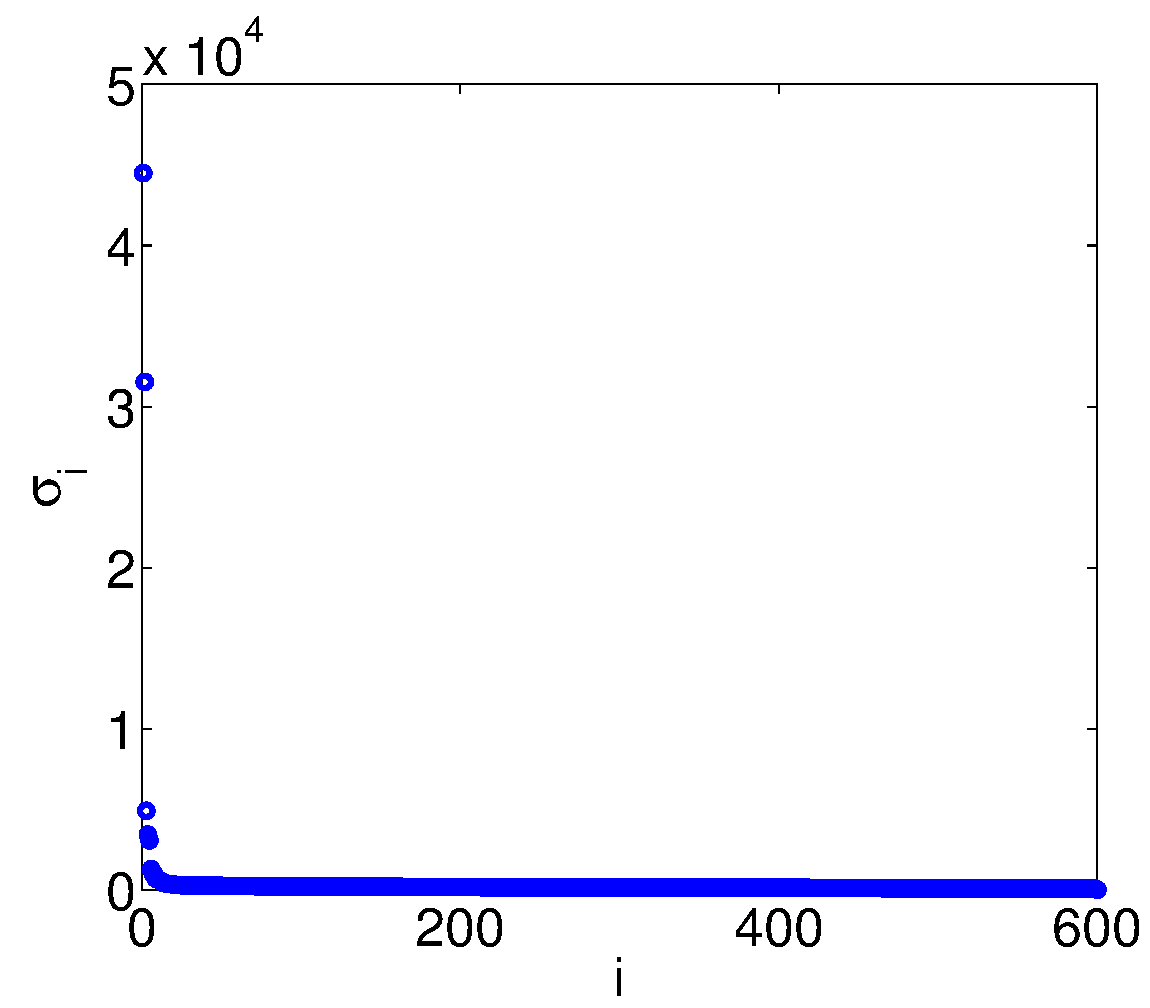
\includegraphics[width=0.3\textwidth]{chpt10_mcca/figs/mcca_msv.pdf}
    }
    \subfigure[Right Camera]{
      \label{fig:chpt10:mcca_right_sv}
      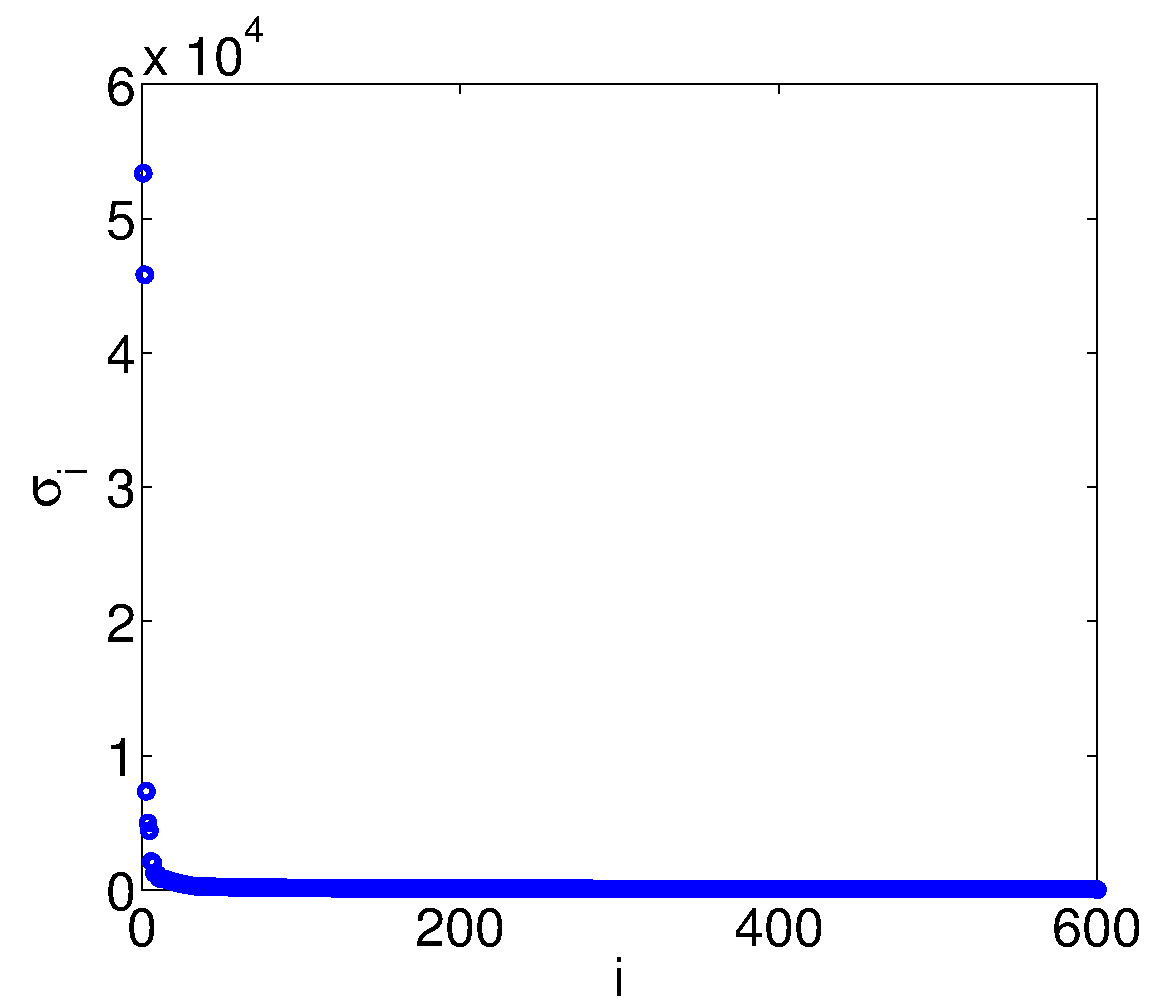
\includegraphics[width=0.3\textwidth]{chpt10_mcca/figs/mcca_rsv.pdf}
    }   
    \caption{Singular value spectra of $Y_{\text{left}}$, $Y_{\text{middle}}$, and $Y_{\text{right}}$}
    \label{fig:chpt10:mcca_svs}
  \end{center}
\end{figure}

\begin{figure}
  \begin{center}
    \subfigure[$u_1$]{
      \label{fig:chpt10:mcca_left_u1}
      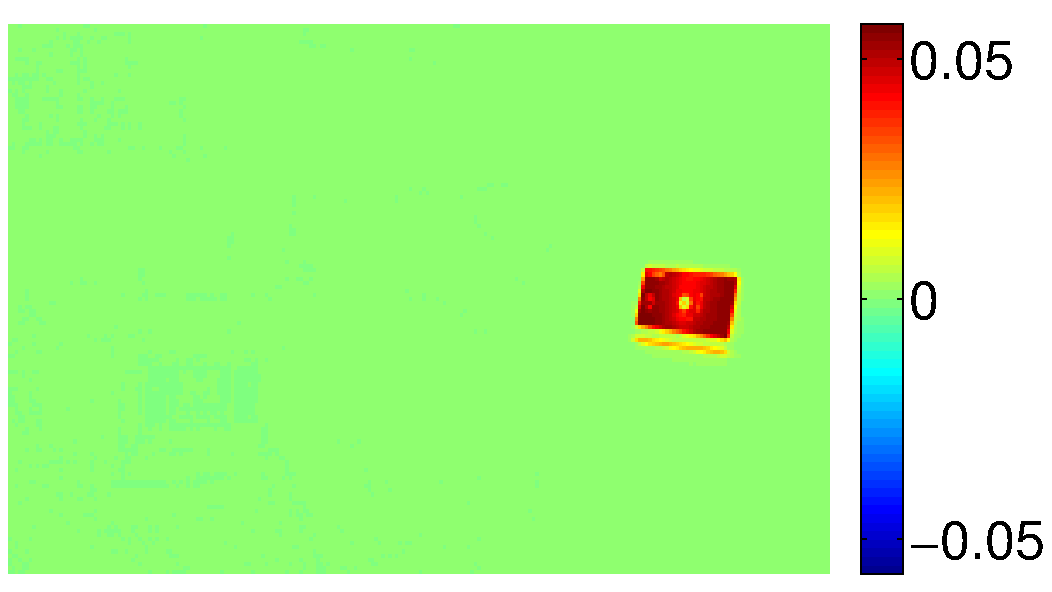
\includegraphics[width=0.4\textwidth]{chpt10_mcca/figs/mcca_ul1.pdf}
    }
    \subfigure[$u_2$]{
      \label{fig:chpt10:mcca_left_u2}
      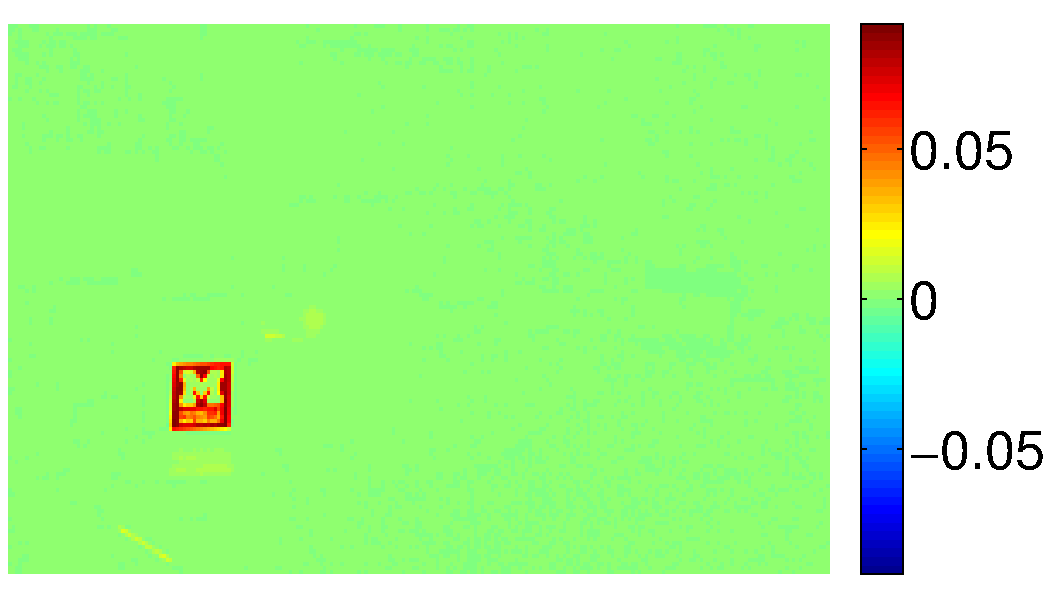
\includegraphics[width=0.4\textwidth]{chpt10_mcca/figs/mcca_ul2.pdf}
    }
    \subfigure[$u_3$]{
      \label{fig:chpt10:mcca_left_u3}
      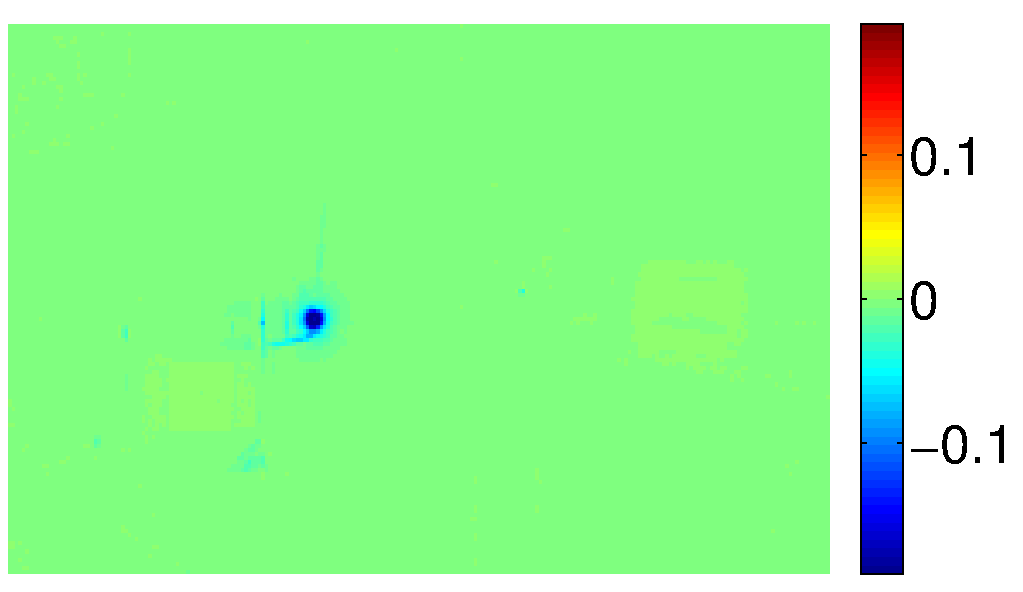
\includegraphics[width=0.4\textwidth]{chpt10_mcca/figs/mcca_ul3.pdf}
    }   
    \subfigure[Overlay]{
      \label{fig:chpt10:mcca_left_overlay}
      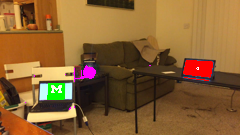
\includegraphics[width=0.4\textwidth]{chpt10_mcca/figs/mcca_left_pca.png}
    }   
    \caption{(a)-(c) Left singular vectors of $Y_{\text{left}}$ corresponding to the top 3
    singular values. (d) Thresholded singular vectors from (a)-(c) overlayed onto the
    original scene. These pixels correspond to the flashing light sources visible in the
    left camera.}
    \label{fig:chpt10:mcca_pca_left}
  \end{center}
\end{figure}

\begin{figure}
  \begin{center}
    \subfigure[$u_1$]{
      \label{fig:chpt10:mcca_mid_u1}
      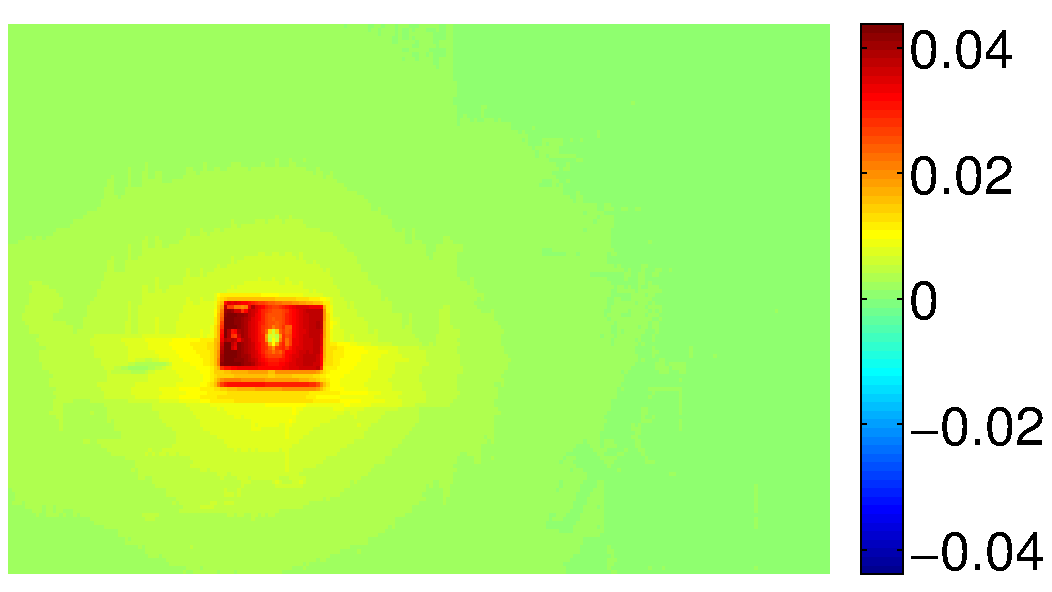
\includegraphics[width=0.4\textwidth]{chpt10_mcca/figs/mcca_um1.pdf}
    }
    \subfigure[Overlay]{
      \label{fig:chpt10:mcca_mid_overlay}
      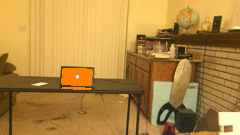
\includegraphics[width=0.4\textwidth]{chpt10_mcca/figs/mcca_mid_pca.png}
    }   
    \caption{(a) Left singular vector of $Y_{\text{middle}}$ corresponding to the top
    singular value. (b) Thresholded singular vector from (a) overlayed onto the
    original scene. These pixels correspond to the flashing light source visible in the
    middle camera.}
    \label{fig:chpt10:mcca_pca_mid}
  \end{center}
\end{figure}

\begin{figure}
  \begin{center}
    \subfigure[$u_1$]{
      \label{fig:chpt10:mcca_right_u1}
      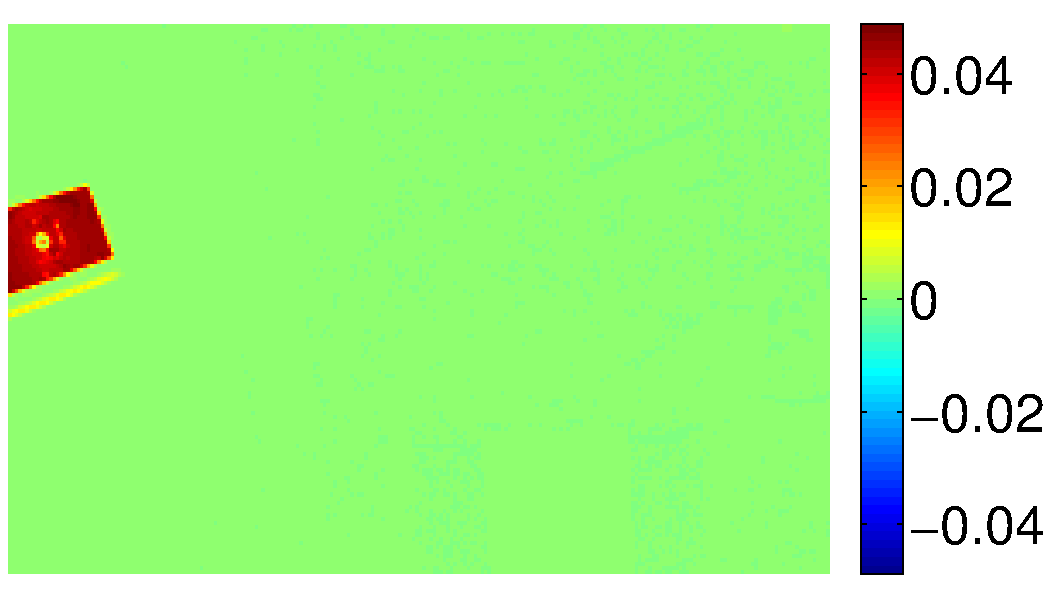
\includegraphics[width=0.4\textwidth]{chpt10_mcca/figs/mcca_ur1.pdf}
    }
    \subfigure[$u_2$]{
      \label{fig:chpt10:mcca_right_u2}
      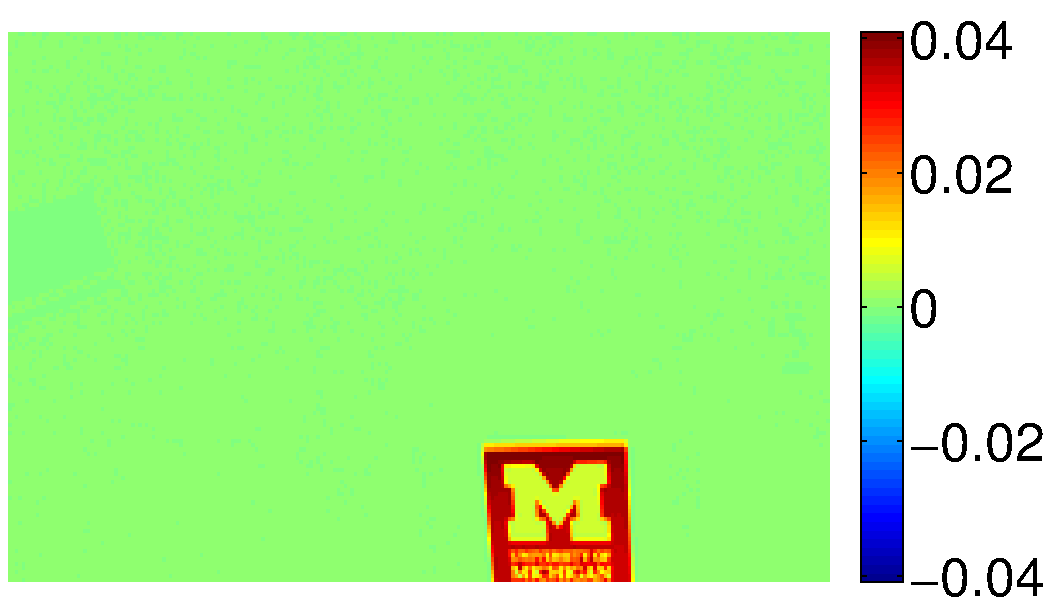
\includegraphics[width=0.4\textwidth]{chpt10_mcca/figs/mcca_ur2.pdf}
    }
    \subfigure[$u_3$]{
      \label{fig:chpt10:mcca_right_u3}
      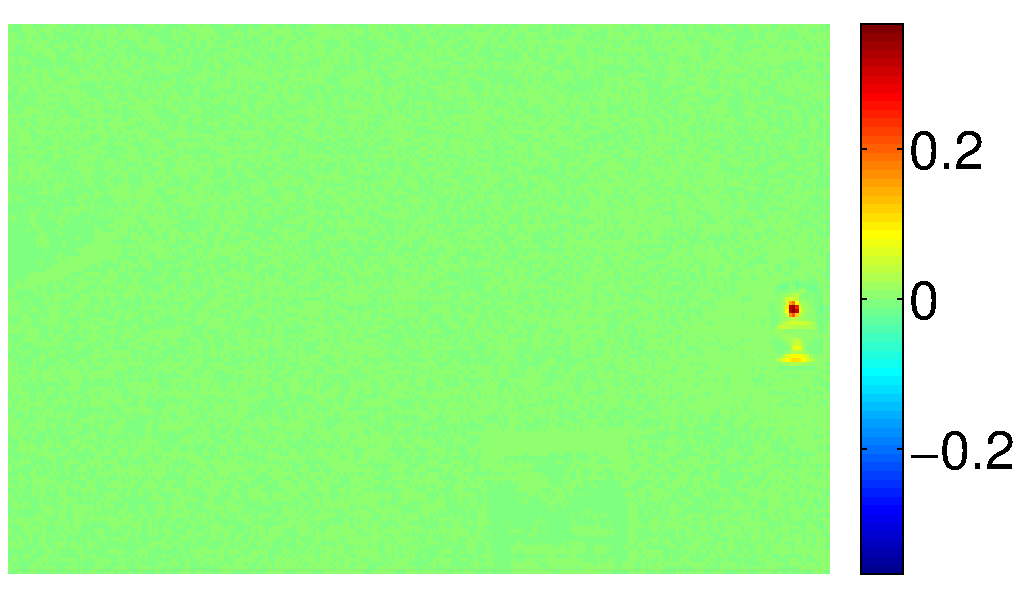
\includegraphics[width=0.4\textwidth]{chpt10_mcca/figs/mcca_ur3.pdf}
    }   
    \subfigure[Overlay]{
      \label{fig:chpt10:mcca_right_overlay}
      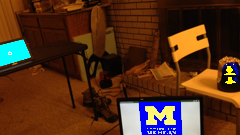
\includegraphics[width=0.4\textwidth]{chpt10_mcca/figs/mcca_right_pca.png}
    }   
    \caption{(a)-(c) Left singular vectors of $Y_{\text{right}}$ corresponding to the top 3
    singular values. (d) Thresholded singular vectors from (a)-(c) overlayed onto the
    original scene. These pixels correspond to the flashing light sources visible in the
    right camera.}
    \label{fig:chpt10:mcca_pca_right}
  \end{center}
\end{figure}

While PCA does a nice job at identifying pixels in each view with a flashing light, it
does not provide any information about whether these pixels are correlated across
cameras. To accomplish this, we turn to MCCA and IMCCA. In an adaptive setting, we can run
these algorithms after every new frame. Specifically, for frame $\ell$, we construct the
$32400\times \ell$ submatrices $Y_{\text{left}}^{\ell}$, $Y_{\text{middle}}^{\ell}$, and
$Y_{\text{right}}^{\ell}$ by taking the matrix of the first $\ell$ original vectorized
frames in each view and then subtracting the mean of the resulting submatrix. We then use these
resulting submatrices as inputs to MCCA and IMCCA. Using our knowledge of the number of
sources in each camera, we set $\widehat{k}_{\text{left}}=3$,
$\widehat{k}_{\text{middle}}=1$, and $\widehat{k}_{\text{right}}=3$. Figure
\ref{fig:chpt10:mcca_corrs} plots the top 3 correlation coefficients returned by MCCA and IMCCA
over the 600 frames of the video. As expected due to our extreme sample deficient regime,
MCCA returns coefficients equal to $2=m-1$. 

\begin{figure}
  \begin{center}
    \subfigure[MCCA]{
      \label{fig:chpt10:mcca_mid_u1}
      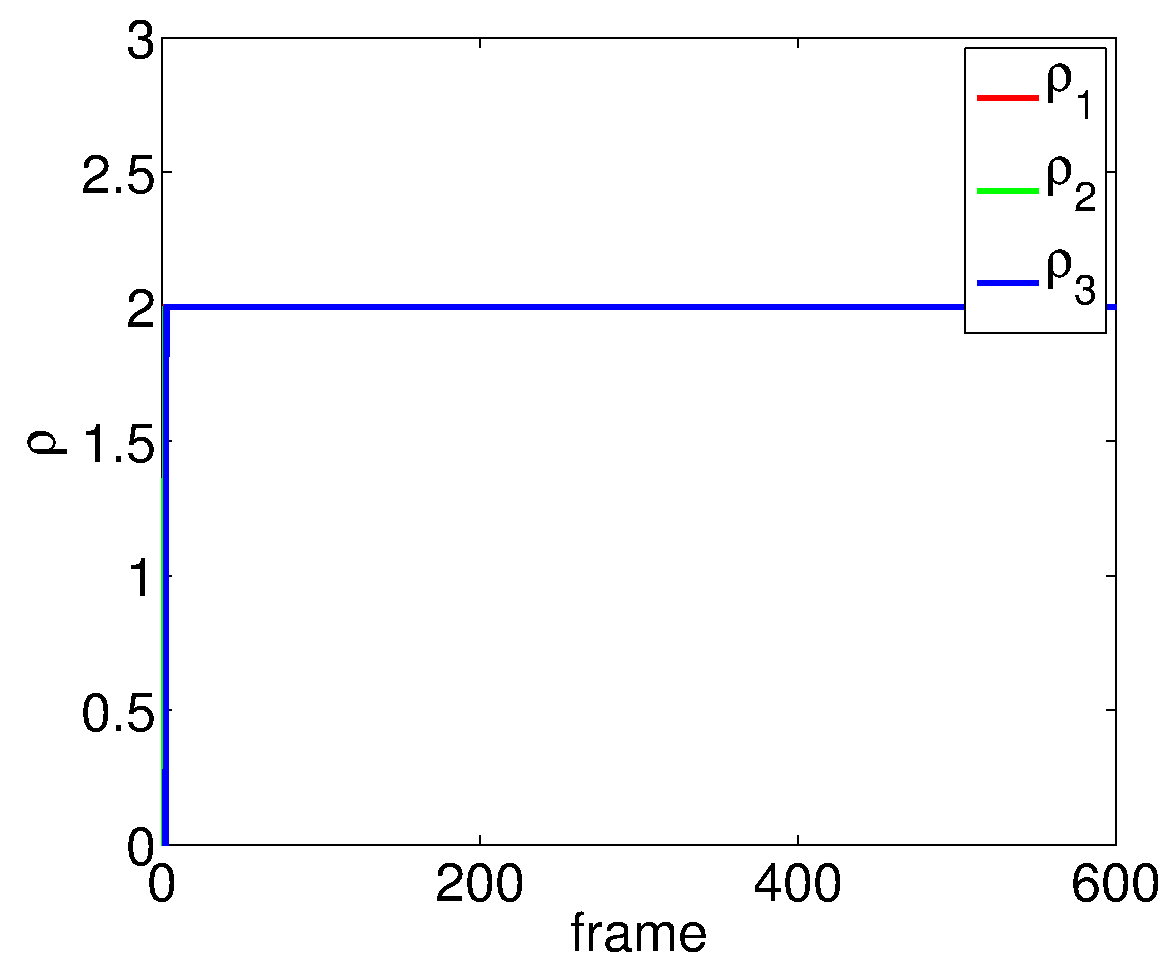
\includegraphics[width=0.4\textwidth]{chpt10_mcca/figs/mcca_cca_corrs.pdf}
    }
    \subfigure[IMCCA]{
      \label{fig:chpt10:mcca_mid_overlay}
      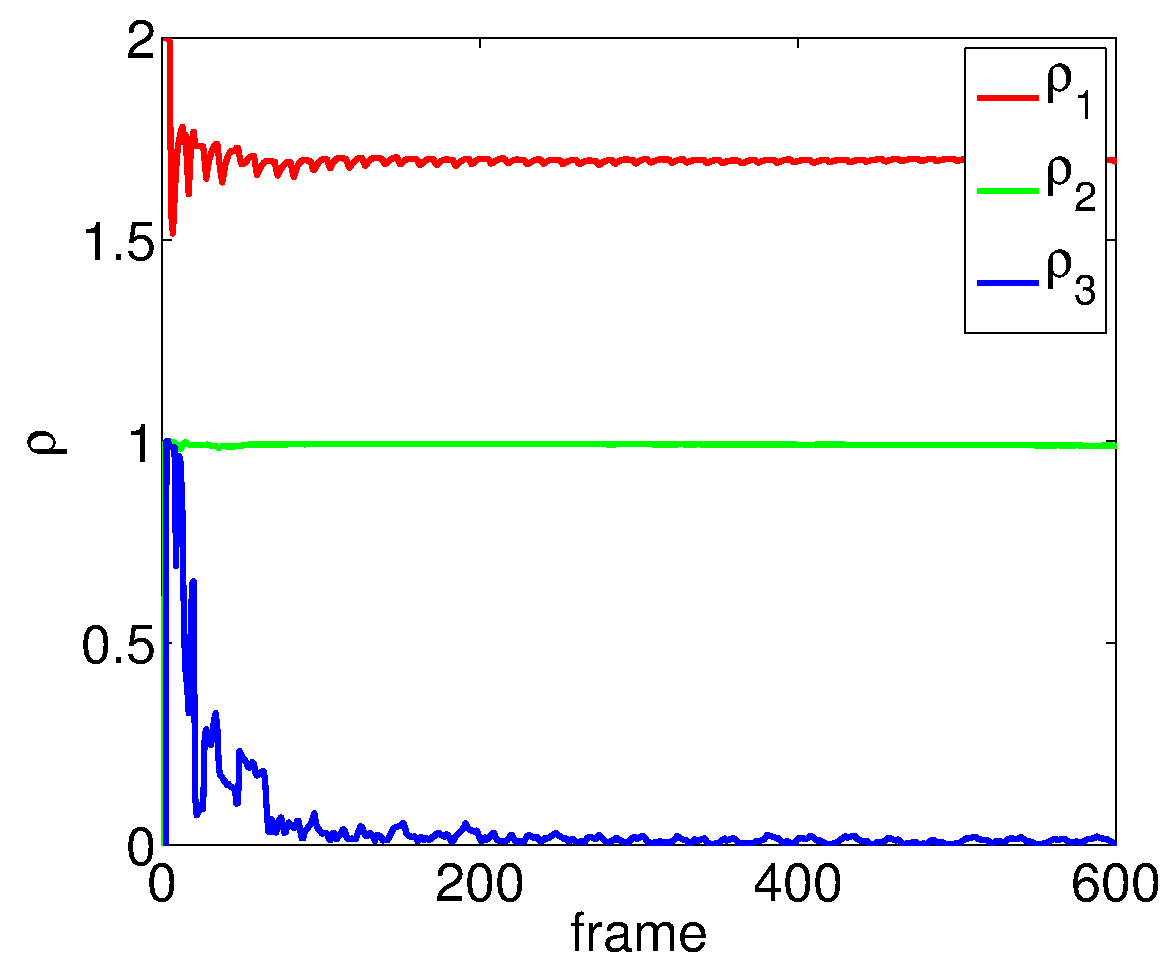
\includegraphics[width=0.4\textwidth]{chpt10_mcca/figs/mcca_icca_corrs.pdf}
    }   
    \caption{Top 3 correlations returned by MCCA and IMCCA.}
    \label{fig:chpt10:mcca_corrs}
  \end{center}
\end{figure}

Figures \ref{fig:chpt10:mcca_cca_vects} and \ref{fig:chpt10:mcca_icca_vects} overlay the thresholded
canonical vectors corresponding to the correlations in Figure \ref{fig:chpt10:mcca_corrs} onto the
original scene for MCCA and IMCCA, respectively. Unsurprisingly, the MCCA canonical
vectors appear extremely random and noisy while the IMCCA canonical vectors correctly
identify the two sources of correlation in our video. Additionally, IMCCA identifies
that once source of correlation appears in all three camera views (red pixels) and that
one source of correlation appears in only two camera views (green pixels). 

To overlay the thresholded canonical correlations on the original scene, we use a
different threshold than $\sqrt{\log(n)/n}$. The main reason for this is that our
eigenvector returned by MCCA is unit norm and contains information for all three canonical
vectors. Therefore, the energy may be dispersed across all views. Consider the following
examples of (possible) canonical vectors returned by IMCCA for our situation of $k=7$ signals,
\be\ba
&u_1 = \left[1/\sqrt{3}, 0, 0, 1/\sqrt{3}, 1/\sqrt{3}, 0, 0 \right]^T\\
&u_2 = \left[0, 1/\sqrt{2}, 0, 0, 0, 1/\sqrt{2}, 0 \right]^T\\
&u_3 = \left[0, 0, 1, 0, 0, 0, 0, \right]^T.\\
\ea\ee
In these examples, the first three components could correspond to the left camera signals,
the fourth component could correspond to the middle camera, and the last three components
could correspond to the right camera. Examining $u_1$, we see that this vector structure
tells us that there is a correlation between all three cameras. Examining $u_2$, this
vector structure tells us that there is a correlation between only the left and right
cameras. Finally, $u_3$ shows that there is no correlation between the cameras. In this
noise-free setting, it is easy to see that components with zero weight are not
correlated. However, in the noisy settings, these non-correlated components will be small but
non-zero. Therefore, we propose the following thresholding technique 
\begin{enumerate}
\item $\widetilde{u}_i = \sqrt{m}u_i$
\item Extract the components for each dataset from $\widetilde{u}_i$, resulting in
  $\widetilde{u}_i^{(j)}$ for $j=1,\dots,m$. 
\item If $\|\widetilde{u}_i^{(j)}\|_2 >1$, then $\widetilde{u}_i^{(j)} = \widetilde{u}_i^{(j)}/\|\widetilde{u}_i^{(j)}\|_2$
\end{enumerate}
The resulting $\widetilde{u}_i^j$ now have at most norm $1$, but uncorrelated components
still remain small. Therefore, using $\widetilde{u}_i^j$ to weight the principal component
vectors, we may use our normal threshold of $\sqrt{\log(d_i)/d_i}$. The above steps are a
heuristic to determine the number of views that a large correlation represents. The worst
case is when all $m$ datasets are correlated and the energy in $u_i$ is distributed evenly
across the $m$ components. The first step accounts for this by scaling all components by
$\sqrt{m}$. In our toy example, the subvectors of $u_1$ each have unit norm for each
dataset. However, in cases where only a subset of the datasets are correlated, as in
$u_2$, this scaling overcompensates and so we use step 2 to make all subvectors at
most unit norm. However as we don't normalize all subvectors, those with small norm will
stay small, correctly indicating their dataset is not correlated.




\begin{figure}
  \begin{center}
    \subfigure[Left Camera]{
      \label{fig:chpt10:mcca_cca_left}
      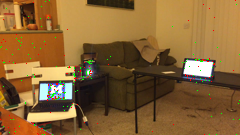
\includegraphics[width=0.3\textwidth]{chpt10_mcca/figs/mcca_left_cca.png}
    }
    \subfigure[Middle Camera]{
      \label{fig:chpt10:mcca_cca_mid}
      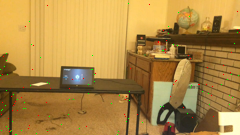
\includegraphics[width=0.3\textwidth]{chpt10_mcca/figs/mcca_mid_cca.png}
    }
    \subfigure[Right Camera]{
      \label{fig:chpt10:mcca_cca_right}
      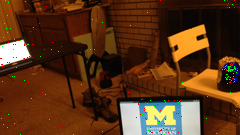
\includegraphics[width=0.3\textwidth]{chpt10_mcca/figs/mcca_right_cca.png}
    }   
    \caption{Top 2 thresholded MCCA canonical vectors overlayed onto the original
      scene. The red pixels are the pixels corresponding to the largest correlation and
      the green pixels correspond to the pixels with the second largest correlation. Since
      we are in the sample deficient regime, MCCA returns random pixels as the canonical
      vectors are random.}
    \label{fig:chpt10:mcca_cca_vects}
  \end{center}
\end{figure}

\begin{figure}
  \begin{center}
    \subfigure[Left Camera]{
      \label{fig:chpt10:mcca_icca_left}
      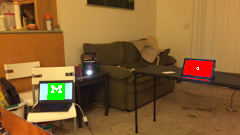
\includegraphics[width=0.3\textwidth]{chpt10_mcca/figs/mcca_left_icca.png}
    }
    \subfigure[Middle Camera]{
      \label{fig:chpt10:mcca_icca_mid}
      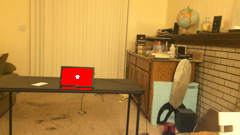
\includegraphics[width=0.3\textwidth]{chpt10_mcca/figs/mcca_mid_icca.png}
    }
    \subfigure[Right Camera]{
      \label{fig:chpt10:mcca_icca_right}
      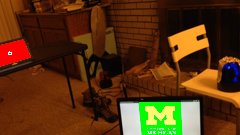
\includegraphics[width=0.3\textwidth]{chpt10_mcca/figs/mcca_right_icca.png}
    }   
    \caption{Top 2 thresholded IMCCA canonical vectors overlayed onto the original
      scene. The red pixels correspond to the largest correlation and the green pixels
      correspond to the second largest correlation. Clearly, the red pixels identify the
      shared flashing tablet light in all 3 views and the green pixels identify the shared
      flashing laptop in the left and right views.}
    \label{fig:chpt10:mcca_icca_vects}
  \end{center}
\end{figure}


